\documentclass[aspectratio=169]{beamer}
\usepackage[T1]{fontenc}
\usepackage[utf8]{inputenc}
\usepackage{listings}
\usepackage{colortbl}

\definecolor{codegreen}{rgb}{0,0.6,0}
\definecolor{codegray}{rgb}{0.5,0.5,0.5}
\definecolor{codepurple}{rgb}{0.58,0,0.82}
\definecolor{backcolour}{rgb}{0.95,0.95,0.92}

\lstdefinestyle{mystyle}{
    backgroundcolor=\color{backcolour},
    commentstyle=\color{codegreen},
    keywordstyle=\color{magenta},
    numberstyle=\tiny\color{codegray},
    stringstyle=\color{codepurple},
    basicstyle=\ttfamily\footnotesize,
    breakatwhitespace=false,
    breaklines=false,
    captionpos=b,
    keepspaces=true,
    numbers=left,
    numbersep=5pt,
    showspaces=false,
    showstringspaces=false,
    showtabs=false,
    tabsize=2
}


\lstdefinestyle{yaml}{
    basicstyle=\color{blue}\footnotesize,
    string=[s]{'}{'},
    comment=[l]{:},
    morecomment=[l]{-}
    backgroundcolor=\color{backcolour},
    commentstyle=\color{codegreen},
    keywordstyle=\color{magenta},
    numberstyle=\tiny\color{codegray},
    stringstyle=\color{codepurple},
    basicstyle=\ttfamily\footnotesize,
    breakatwhitespace=false,
    breaklines=false,
    captionpos=b,
    keepspaces=true,
    numbers=left,
    numbersep=5pt,
    showspaces=false,
    showstringspaces=false,
    showtabs=false,
    tabsize=2
 }

\lstset{style=mystyle}

\title{Warewulf\\
making cluster\\
installations fast and \\
reliable}
\date{April 25, Ostrava}
\author{Christian Goll <\texttt{cgoll@suse.com}>}
\usetheme{suse}

\begin{document}

\begin{frame}
\titlepage
\end{frame}
\begin{frame}[fragile]
\frametitle{Introduction}
\framesubtitle{Warewulf is tool for managing beowulf clusters}
\begin{columns}
\column{0.5\textwidth}
\begin{block}{Beowulf}
  \begin{itemize}
    \item old british poem
  \end{itemize}
\end{block}
\begin{block}{Beowulf cluster}
  \begin{itemize}
    \item became popular in the 90.
    \item use of the shelf hardware
    \begin{itemize}
      \item 486 \& linux
      \item \textbf{not} Cray \& unix
    \end{itemize}
    \item warewulf is a typo of werewolf
  \end{itemize}
\end{block}
\column{0.5\textwidth}
  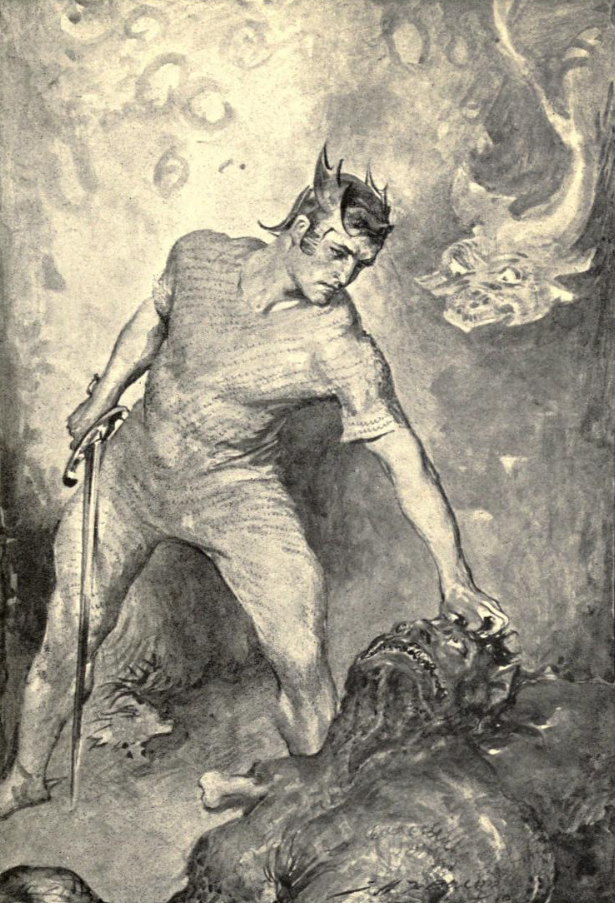
\includegraphics[width=.6\linewidth]{Beowulf}
\end{columns}
\end{frame}

\begin{frame}[fragile]
\frametitle{Introduction}
\framesubtitle{HPC landscape}
\begin{block}{Top five Supercomputers}
\begin{table}
\begin{tabular}{c|l|l|l|l}
1 &	Frontier& EPYC 64C &AMD MI250X &Slingshot-11 \\
2 &	Aurora  & Xeon 9470 & Intel GPU Max&Slingshot-11 \\
3 &	Eagle & Xeon 8480 &  NVIDIA H100 & NVIDIA Infiniband \\
\rowcolor{backcolour}
4 &	Fugaku &  A64FX 48C 2.2GHz & - & Tofu interconnect D \\
5 &	LUMI &  EPYC 64C 2GHz & AMD MI250X & Slingshot-11 
\end{tabular}
\end{table}
\begin{itemize}
  \item only Fugaku uses non standard CPU
  \item others are beowulf clusters with GPUs attached
\end{itemize}
\end{block}
\end{frame}
\begin{frame}[fragile]
\frametitle{Introduction}
\framesubtitle{Beowulf cluster}
\begin{columns}
\column{0.5\textwidth}
\begin{block}{base components}
\begin{itemize}
  \item management node
  \item compute nodes
  \item management network
\end{itemize}
\end{block}
\begin{block}{optional components}
\begin{itemize}
  \item more compute nodes
  \item fast network interconnects 
  \item central storage
  \item bmc/ipmi
\end{itemize}
\end{block}
\column{0.5\textwidth}
  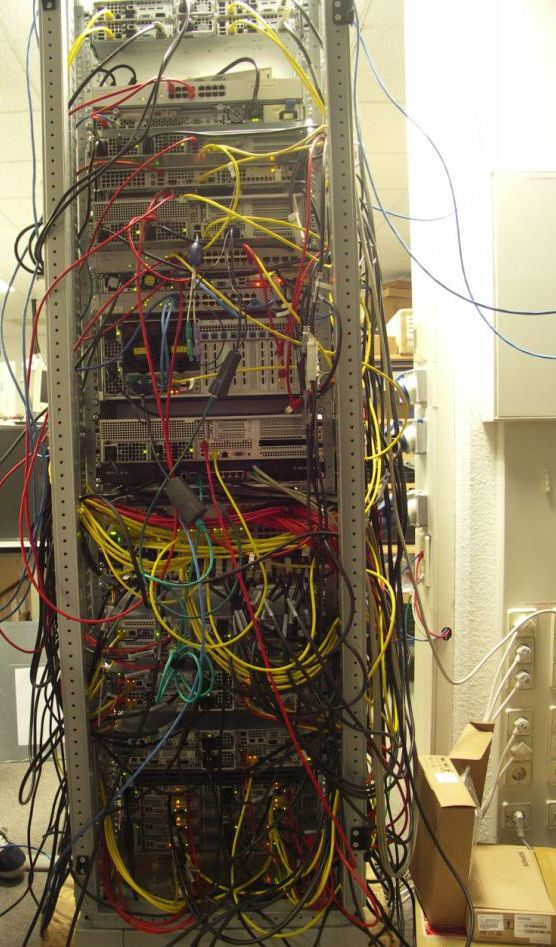
\includegraphics[width=.6\linewidth]{Transtec-056}
\end{columns}
\end{frame}
\begin{frame}[fragile]
\frametitle{Introduction}
\framesubtitle{Beowulf Cluster}
\begin{columns}
\column{0.5\textwidth}
\begin{block}{differences to data centers}
  \begin{itemize}
    \item compute nodes are cattle
    \item hierarchical organization
    \item compute are not updated after boot process
    \item application come from central storage
    \item applications are self compiled
    \item one application can run over several nodes
  \end{itemize}
\end{block}
\column{0.5\textwidth}
  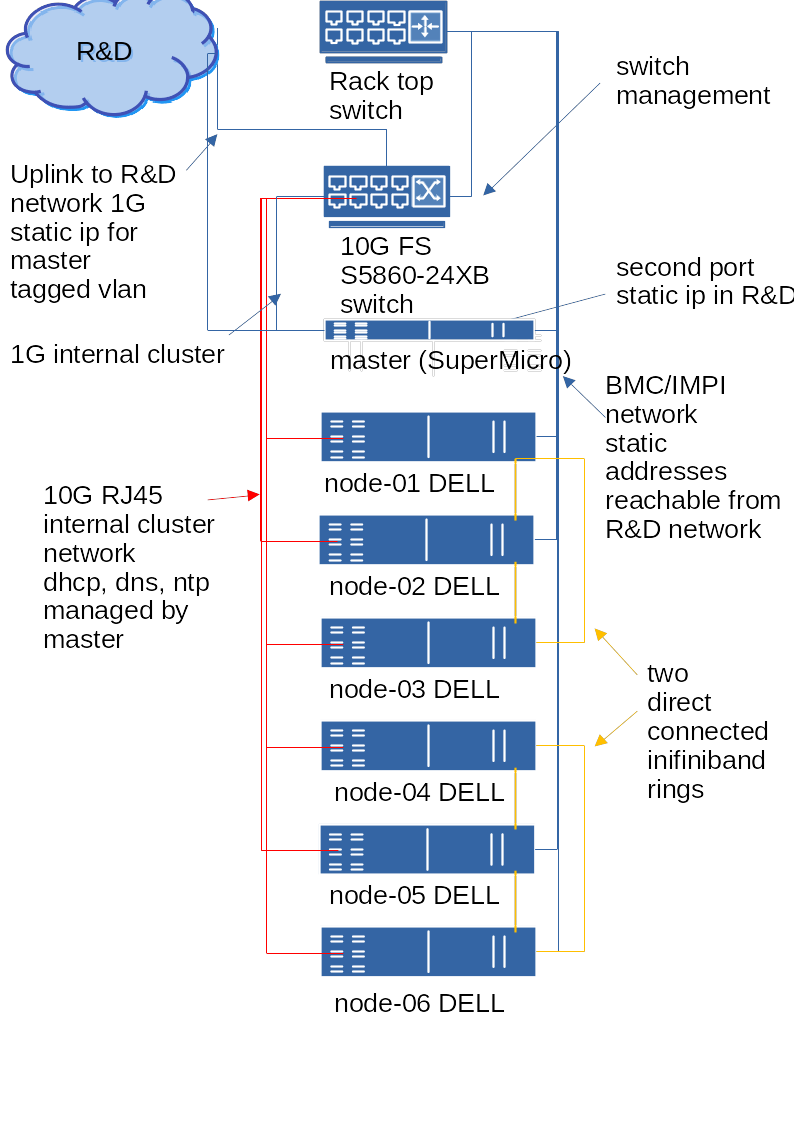
\includegraphics[width=.6\linewidth]{networkplan}
\end{columns}
\end{frame}
\begin{frame}[fragile]
\frametitle{Warewulf description}
\framesubtitle{software stack}
\begin{columns}
\column{0.5\textwidth}
  \begin{block}{warewulf components}
  \hspace*{.1\linewidth}\begin{minipage}{.8\linewidth}
  \begin{block}{warewulfd delivers}
    \begin{itemize}
      \item kernel \& modules
      \item node image
      \item node configurations
    \end{itemize}
  \end{block}
  \begin{block}{\texttt{wwctl} cmd line tool}
    \begin{itemize}
      \item manages node database
      \item manages node image
    \end{itemize}
  \end{block}
  \vspace*{1cm}
  \end{minipage}
  \end{block}
\column{0.5\textwidth}
  \begin{block}{external components}
  \hspace*{.1\linewidth}\begin{minipage}{.8\linewidth}
    \begin{block}{dhcp server}
      \begin{itemize}
      \item ISC dhcpd server
      \item dnsmasq
    \end{itemize}
    \end{block}
    \begin{block}{tftp}
      \begin{itemize}
      \item kernel tftp
      \item dnsmasq
    \end{itemize}
    \end{block}
  \end{minipage} 
  \end{block}
  \begin{block}{optional}
    \begin{itemize}
      \item nfs
      \item manage \texttt{/etc/hosts}
    \end{itemize}
  \end{block}
\end{columns}
\end{frame}

\begin{frame}[fragile]
\frametitle{Warewulf description}
\framesubtitle{database \texttt{/etc/warewulf/nodes.conf}}
\begin{columns}
%
\column{0.5\textwidth}
\begin{itemize}
\item plain yaml file
  \item easy backup
  \item can be version controlled
  \item external tools support
  \begin{itemize}
    \item vim, ansible
  \end{itemize}
\end{itemize}
\begin{block}{profiles}
\begin{itemize}
  \item stores identical values for collection of nodes
  \item values can be overiden on node basis
\end{itemize}
\end{block}
\column{0.5\textwidth}
\begin{lstlisting}[style=yaml]
WW_INTERNAL: 45
nodeprofiles:
  default:
    comment: This profile is automatically included for each node
    container name: leap
    network devices:
      default:
        device: eth0
nodes:
  n01:
    profiles:
    - default
    network devices:
      default:
        hwaddr: 52:54:00:4e:cb:1d
        ipaddr: 172.16.130.101
  n02:
\end{lstlisting}
%
\end{columns}
\end{frame}
\begin{frame}[fragile]
\frametitle{Warewulf description}
\framesubtitle{command line database manipulation}
\begin{columns}
\column{0.25\textwidth}
\begin{block}{add node}
\texttt{wwctl node add n01 -I 10.10.10.1}
\end{block}
\begin{block}{modify node}
\texttt{wwctl node set n01 --comment "Have fun"}
\end{block}
\begin{block}{list node}
\texttt{wwctl node list n01 -a"}
\end{block}
\vspace*{3cm}
\column{0.75\textwidth}
\begin{lstlisting}[style=mystyle]
NODE FIELD                    PROFILE    VALUE
n01  Id                       --         n01
n01  Comment                  SUPERSEDED Have fun
n01  ContainerName            default    leap
n01  Ipxe                     --         (default)
n01  RuntimeOverlay           --         (generic)
n01  SystemOverlay            --         (wwinit)
n01  Root                     --         (initramfs)
n01  Discoverable             --         false
n01  Init                     --         (/sbin/init)
n01  Kernel.Args              --         (quiet crashkernel=no vga=791 net.naming-scheme=v238)
n01  Profiles                 --         default
n01  PrimaryNetDev            --         (default)
n01  NetDevs[default].Type    --         (ethernet)
n01  NetDevs[default].OnBoot  --         (true)
n01  NetDevs[default].Device  default    eth0
n01  NetDevs[default].Hwaddr  --         52:54:00:4e:cb:1d
n01  NetDevs[default].Ipaddr  --         172.16.130.101
n01  NetDevs[default].Netmask --         (255.255.255.0)
n01  NetDevs[default].Primary --         (true)
\end{lstlisting}
\end{columns}
\end{frame}
%
%
%\frametitle{Presentation Title}
%\framesubtitle{This is \textit{a subtitle}.}
%
%\begin{columns}
%
%\column{0.5\textwidth}
%This is a text in first column.
%\begin{itemize}
%  \item First item
%  \item Second item
%  \item \texttt{mono spaced font example}
%  \begin{itemize}
%    \item First item
%    \item Second item
%  \end{itemize}
%\end{itemize}
%
%\column{0.5\textwidth}
%This text will be in the second column
%and on a second thought this is a nice looking
%layout in some cases.
%
%\begin{lstlisting}[language=C, caption=C example]
%#include <stdio.h>
%
%/* some comment */
%int main() {
%  printf("Hello World");
%}
%\end{lstlisting}
%
%\end{columns}
%
%\end{frame}
%
%\begin{frame}
%\frametitle{Another slide}
%\framesubtitle{This is \textit{a subtitle}.}
%
%\begin{table}
%  \begin{tabular}{c|c}
%    table1 & trial \\
%    \hline
%    \hline
%    1 & 2 \\
%    3 & 4
%  \end{tabular}
%  \caption*{My table}
%\end{table}
%\end{frame}
%
\end{document}

